\section{Введение}
\label{sec:Chapter0} \index{Chapter0}
\subsection{Введение в область}
История развития методов машинного обучения начинается с середины 20-го века с появления первых алгоритмов, таких как линейная регрессия и метод наименьших квадратов. Со временем методы усложнялись, и в 1980-х и 1990-х годах были разработаны нейронные сети и методы обратного распространения ошибки, что заложило основу для глубокого обучения. С начала 2000-х годов рост вычислительных мощностей и доступность больших данных ускорили прогресс в машинном обучении. Появление графических процессоров (GPU) и специализированных аппаратных решений позволило обучать глубокие нейронные сети на больших объемах данных, что привело к прорывам в распознавании образов, обработке естественного языка и хемоинформатике. 
% В хемоинформатике методы машинного обучения стали важны благодаря способности обрабатывать большие объемы данных и выявлять закономерности в молекулярных структурах. 
% Первоначально использовавшиеся методы, такие как квантово-механические расчеты и молекулярная динамика, хотя и были точными, требовали значительных вычислительных ресурсов и времени.
Благодаря своей способности обрабатывать большие объемы данных и выявлять закономерности в молекулярных структурах, введение машинного обучения в хемоинформатике позволило значительно ускорить процесс анализа и предсказания молекулярных свойств, сделав его более эффективным и доступным.

В последние годы методы машинного обучения, особенно те, что основаны на глубоком обучении, демонстрируют значительные успехи в области хемоинформатики и физической химии. Однако ограниченность данных является основной проблемой для обучения моделей, так как каждый экспериментальный результат требует значительных лабораторных усилий. Это ставит химию в контраст с такими областями, как компьютерное зрение или обработка естественного языка, где данные более доступны.

Предсказание свойств молекул является актуальной задачей, поскольку молекулы являются базовыми единицами, на свойствах которых основываются дальнейшие исследования реакций, кристаллов и других химических процессов. Молекулы могут быть представлены в виде нескольких форматов. Например, в виде молекулярного графа, где узлы — это атомы, а рёбра — связи между ними (рис. \ref{fig:molecules}). Этот интуитивно понятный способ визуализации намекает на перспективность использования графовых нейронных сетей (GNN) для анализа и предсказания молекулярных свойств. Очень популярным остается строковое представление химических структур SMILES (Simplified Molecular Input Line Entry System) \cite{SMILES}. Основными преимуществами SMILES являются его простота и удобство в использовании. Также, путём обхода графа в глубину и ряда других правил молекула может быть представлена в виде так называемого молекулярного фингерпринта (FP). В данной работе используется улучшенная версия Morgan Finger Print под названием ECFP (Extended-Connectivity Fingerprints) \cite{ECFP}. Эти представления позволяют использовать различные модели для анализа и предсказания молекулярных свойств.
\begin{figure}[h]
\begin{minipage}{0.33\textwidth}
  \centering
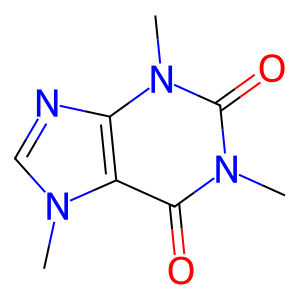
\includegraphics[width =  \textwidth ]{Bachelor-Thesis-Template/images/molecules/molecule1.png}
\end{minipage}%
\begin{minipage}{0.33\textwidth}
  \centering
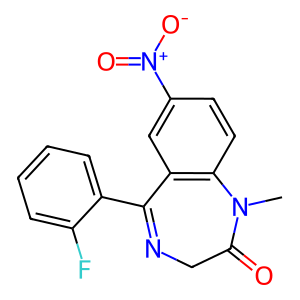
\includegraphics[width =  \textwidth ]{Bachelor-Thesis-Template/images/molecules/molecule2.png}
\end{minipage}%
\begin{minipage}{0.33\textwidth}
  \centering
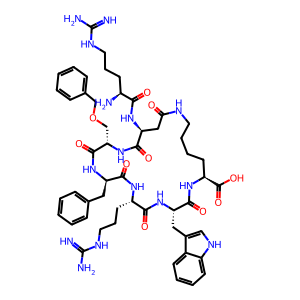
\includegraphics[width =  \textwidth ]{Bachelor-Thesis-Template/images/molecules/molecule3.png}
\end{minipage}%
\newline
\begin{minipage}{0.33\textwidth}
  \centering
(a)
\end{minipage}%
\begin{minipage}{0.33\textwidth}
\centering
 (b)
\end{minipage}%
\begin{minipage}{0.33\textwidth}
\centering
  (c)
\end{minipage}%
\caption{\small Графовые представления молекул.}
    \label{fig:molecules}
\end{figure}


\subsection{Исследование существующих решений}

В рамках исследования существующих методов предсказывания молекулярных свойств и получения эмбеддингов молекул были рассмотрены различные подходы, включая mol2vec \cite{mol2vec}, ChemBERTa \cite{ChemBERTa-2}, SMILES-BERT \cite{SMILESBERT} и другие. Эти методы основаны на принципах обработки естественного языка и используются для преобразования молекулярных структур в векторные представления, которые могут служить входными данными для алгоритмов машинного обучения.
\begin{itemize}
    \item Mol2vec \cite{mol2vec} — это метод, аналогичный Word2Vec в NLP, который использует необученный подход для получения векторных представлений молекулярных подструктур. Он преобразует молекулы в “предложения” и обучает модель на этих данных, что позволяет создавать векторы для новых молекул. Однако, он может столкнуться с ограничениями при работе с более сложными молекулярными структурами.

    \item ChemBERTa \cite{ChemBERTa-2} — это модель, которая использует трансформеры для предсказания свойств молекул. Она была одной из первых попыток систематически оценить трансформеры на задачах предсказания молекулярных свойств. ChemBERTa показала хорошие результаты при предварительном обучении на больших наборах данных и предоставила конкурентоспособную производительность на MoleculeNet \cite{moleculenet}, а также полезные визуализации на основе внимания. Однако, как и другие модели, основанные на трансформерах, она может требовать значительных вычислительных ресурсов.

    \item SMILES-BERT \cite{SMILESBERT} — это подход, который применяет модели BERT к данным SMILES для дизайна лекарств, химического моделирования и предсказания свойств. Этот подход использует предварительно обученные модели на различных наборах данных, таких как ZINC \cite{zinc} и PubChem \cite{pubchem}, и предоставляет веса модели для использования через библиотеку HuggingFace. Однако, использование SMILES как входных данных может привести к потере структурной информации, так как одна и та же молекула может быть представлена различными SMILES-строками.
\end{itemize}
Однако, несмотря на их потенциал, эти методы сталкиваются с определёнными ограничениями, особенно при использовании SMILES как входных данных. SMILES содержит только структурную информацию о молекуле, а также, как было упомянуто выше, одна и та же молекула может быть представлена различными SMILES-строками, что может затруднить обучение моделей и снизить точность предсказаний.

Важно отметить, что выбор метода зависит от конкретной задачи и доступных ресурсов. Например, если вам доступны большие вычислительные ресурсы, ChemBERTa может быть хорошим выбором. Если же вам нужно быстро получить векторные представления молекул, Mol2vec может быть более подходящим решением. В любом случае, все эти методы представляют собой важные инструменты в области химического моделирования и предсказания молекулярных свойств.

\subsection{Цель работы}

Целью данной работы является разработка и тестирование методов дообучения (fine-tuning) моделей трансформеров для предсказания молекулярных свойств на небольших специализированных выборках. Для достижения этой цели используются современные технологии и модели, такие как RoBERTa и MolCLR.

RoBERTa (Robustly optimized BERT approach) \cite{liu2019roberta} представляет собой улучшенную версию модели BERT, которая демонстрирует высокую эффективность в задачах обработки текста и анализа последовательностей, таких как ECFP. MolCLR (Molecular Contrastive Learning of Representations) \cite{molclr} использует метод контрастивного обучения, который позволяет моделям лучше понимать взаимосвязи между молекулярными структурами и их свойствами.

Особое внимание в данной работе уделено объединению моделей RoBERTa и MolCLR, что позволяет использовать преимущества обеих технологий. RoBERTa обеспечивает качественную обработку последовательностей, а MolCLR улучшает представление молекулярных структур через контрастивное обучение. Такое объединение позволяет значительно повысить точность предсказаний и улучшить обобщающую способность моделей.

Кроме того, в работе рассматривается возможность замены MolCLR на Graphormer, так как он лучше справляется с предсказанием свойств молекул. Graphormer сочетает преимущества графовых нейронных сетей и трансформеров, что позволяет более точно предсказывать свойства молекул, особенно для сложных молекулярных структур.

В рамках исследования проводится обучение модели Graphormer и сравнение её с MolCLR на задаче регрессии молекулярного свойства Molecular Weight. Это позволяет оценить эффективность Graphormer в сравнении с MolCLR и определить, какой подход является более оптимальным для предсказания молекулярных свойств.

Основной вклад данной работы заключается в предложении нового подхода к обучению моделей с использованием комбинированных представлений молекул, что позволяет повысить точность предсказаний на небольших выборках данных. Это исследование открывает новые возможности для эффективного применения машинного обучения в хемоинформатике и физической химии.



% Исторический контекст и значимость темы:

% История развития: Кратко опишите, как эволюционировали методы машинного обучения и почему они стали важными в хемоинформатике.
% Значимость исследования: Подчеркните, почему исследование предсказания молекулярных свойств является актуальным и какие потенциальные применения могут быть у результатов этого исследования.
% Текущие вызовы и проблемы:

% Ограниченность данных: Упомяните сложности, связанные с недостатком размеченных данных для обучения моделей, и как ваша работа стремится преодолеть эти ограничения.
% Точность предсказаний: Опишите, какие проблемы существуют с текущими моделями
\newpage
